\documentclass[oribibl]{llncs}
\pagestyle{headings} %page numbers
\usepackage{makeidx}  % allows for indexgeneration
\usepackage[utf8]{inputenc}
\usepackage{pdfpages}
\usepackage{float}
\usepackage{enumitem}
\usepackage[T1]{fontenc} % Fixed missing font warning for \maketitle
\usepackage{url}
\usepackage{todonotes} % remove later - this is for TODO notes
%\usepackage{amsmath,amssymb}  We don't use this?
\usepackage{coqdoc}
\usepackage{url}

\hypersetup{%
  citecolor=black
}

\bibliographystyle{plain}

\begin{document}
\mainmatter
\title{Formal Verification of B+ Trees}
\author{Nicolai Dahl Blicher-Petersen \and Christian Harrington \and Morten Fangel Jensen \\
\email{\{ndbl, cnha, mfan\}@itu.dk}}
\institute{IT University of Copenhagen, Rued Langgaards Vej 7, 2300 Copenhagen S, Denmark}

\maketitle

\begin{abstract}
The B+ tree data structure is a balanced, n-ary tree, used most often in database and file system storage. It is known for its high fanout, thereby minimizing the number of costly I/O operations. Using the Coq interactive proof assistant we define an inductive data type describing a valid B+ tree, used to formally verify properties of the search and insert operations of the data structure. Furthermore, we describe the need for an added level of indirection in the form of an intermediate proposition when proving relations between the insert and search operations.

\keywords{B+ tree, Coq, Gallina}
\end{abstract}

%!TEX root = ../BPlusTree-report.tex
\section{Introduction}
\label{sec:Introduction}
%!TEX root = ../BPlusTree-report.tex
\section{Background}
\label{sec:Background}
% Notes:
% What is a bplustree:
%   - Inherently imperative data structure
%   - Suboptimal implementation
%     - Running time of optimal implementation
%     - Running time of our implementation
%       - Mention how one could make it optimal.
%       - A tree in a tree in a tree, dawg
%     - Running time out of scope

\subsection{Gallina}
Gallina is a purely functional language\todo{ref}, which is used by the Coq interactive proof assistant. It is very lean, and does not include non-functional data structures, such as arrays\todo{ref}.

\subsection{B+ tree}
\label{subsec:Background_Bplus_tree}
The B+ tree is a n-ary, self-balancing, tree data structure\,\cite[pp. 334]{ramakrishnan2003database}, similar to a B-tree. It is composed of a root, nodes, and leaves. The root may be a leaf or a node. Nodes hold pairs of keys and pointers, $(k, p)$. $P$ points to either a node or leaf that holds the values over $k$, but below the key of the next pair. Leaves hold pairs of keys and values, $(k, v)$. In this project keys are always natural numbers, while values can have any type, denoted by $X$. Duplicate keys are not allowed. A typical B+ tree can be seen in Fig. \ref{fig:bplustree}.

\begin{figure}
 \centering
   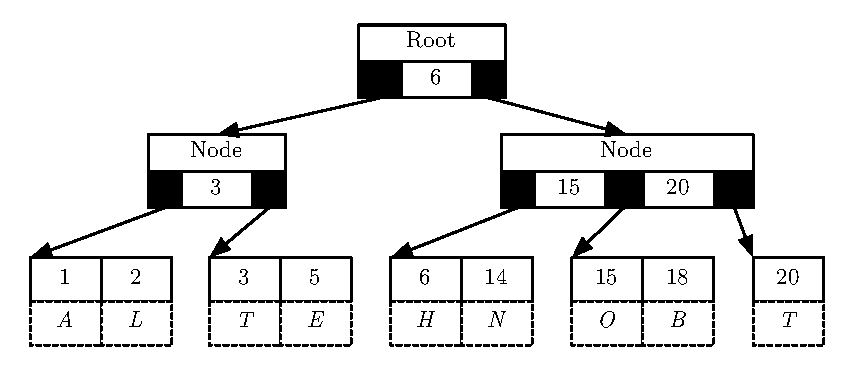
\includegraphics[width=90mm]{diagrams/BPlusTree.pdf}
 \caption{An example of a B+ tree with $b=1$. The bottom row contains leaves, with values, in this case characters, in the dashed boxes.}
 \label{fig:bplustree}
\end{figure}

For a given B+ tree, an order $b$ determines the capacity of nodes and leaves. A root node must have between 2 and $2b+1$ children, while a root leaf must have between + $2b$ values. The constraint is tighter for nodes and leaves which are not the root. An internal node must have between $b+1$ and $2b+1$ children, while non-root leaves must have between $b$ and $2b$ values\,\cite[p. 335]{ramakrishnan2003database}. 

\paragraph{}
In our implementation, a node is a list of key-pointer $(k, p)$ pairs where $p$ points to a child tree. A leaf is a list of key-value $(k, v)$ pairs. We support three operations, which we will refer to as our primary operations. These are: $insert$, $search$ and $height$. The theory behind the $height$ function is trivial, and will not be explained in this section, but the theory behind the $insert$ and $search$ functions require some explanation. In most B+ tree implementations, each leaf is joined to the next leaf by a pointer, allowing fast sequential access to values, which is useful for range queries. To simplify the B+ tree data structure, this has been omitted, and sequential access to values is implemented through a simple in-order traversal of the B+ tree. Likewise, the deletion function is beyond the scope of this project, as the work required for just the $insert$ and $search$ functions is substantial.

\subsubsection{Search}
\label{subsec:Search}
\todo{this section must contain a better discussion of the asymptotic complexity. Why is the running time logb(n)? Because you can do binary search in node keys.}
The $search$ function takes two arguments: a search key $sk$, and a tree $t$, to search in. Tree can be either a node or a leaf. If the the tree is a node, the function finds the pointer $p$ in the node for which it holds that
\begin{itemize}
	\item $p$ is the start pointer of the node and there exists a key $k$ that immediately succeeds $p$, where $sk < k$ OR
	\item There exists keys $k1$ and $k2$ on each side of $p$ and $k1 <= sk < k2$ OR
	\item $p$ is the end pointer of the node and for all keys $k$ in the node $k <= sk$
\end{itemize}
The function then recursively calls itself with the subtree $p$. Once the function reaches a leaf, the function searches for the key-value pair. This is often implemented as binary search in an array. This results in a time complexity of $O(log_b n)$.

\subsubsection{Insert}
The $insert$ function takes two arguments: a key-value pair $(k, v)$ and a tree $t$ to insert the pair into. The function starts at the root of the tree, and recursively searches for the leaf to insert into. It does this search in the same way the Search operation does it. The pair is then inserted into the leaf at the correct position. If the insertion results in the leaf having more than $2b$ values, the leaf must be split. This is called a leaf overflow. This is handled by splitting the leaf in half, and inserting a pointer to the new leaf in the parent node. If the parent node now has more than $2b$ children, it most also be split, following the same pattern. This can continue all the way to the root, which in turn can be split into two. If this happens, a new root node is created, as a parent to two split halves of the old root, and the height of the tree increases by one. Thus, a B+ tree can be seen to grow up from the leaves and is always in perfect balance. The complexity of such an $insert$ function is $O(log_b n)$.

%!TEX root = ../BPlusTree-report.tex
\section{Problem Analysis}
\label{sec:ProblemAnalysis}
% Notes:
% Relevant constructs
%   - bplustree
%   - insert
%   - search 
%   - height
%   - deletion
% We want to prove:
%   - Insert works
%     - Inductive data types
%       - valid_bplus_tree
%       - appears_in_kvl
%       - appears_in_tree
%       - kvl_sorted
%     - Works under these assumptions...
%       -Valid bplustree
%       - Insertion preserves tree
%   - Search works
To implement B+ trees in Gallina, several different components have to be implemented. Most importantly, we must specify an inductive data type that describes a B+ tree, which can be seen in Figure \ref{fig:inductive_data_type}.

\begin{figure}
\centering
\begin{coqdoccode}
\coqdockw{Inductive} \coqdocvar{bplustree} (\coqdocvar{b}: \coqdocvar{nat}) (\coqdocvar{X}:\coqdockw{Type}) : \coqdockw{Type} :=\coqdoceol
\coqdocindent{1.00em}
\ensuremath{|} \coqdocvar{bptLeaf} : \coqdocvar{list} (\coqdocvar{nat} \ensuremath{\times} \coqdocvar{X}) \ensuremath{\rightarrow} \coqdocvar{bplustree} \coqdocvar{b} \coqdocvar{X}\coqdoceol
\coqdocindent{1.00em}
\ensuremath{|} \coqdocvar{bptNode} : \coqdocvar{list} (\coqdocvar{nat} \ensuremath{\times} (\coqdocvar{bplustree} \coqdocvar{b} \coqdocvar{X})) \ensuremath{\rightarrow} \coqdocvar{bplustree} \coqdocvar{b} \coqdocvar{X}.\coqdoceol
\end{coqdoccode}
\caption{Inductive data type for B+ tree.}
\label{fig:inductive_data_type}
\end{figure}

\paragraph{}
This data type says that a $bplustree$ is parameterized by $b$, the order, and $X$, the type of the values in the tree. Further, a tree can be either a leaf or a node. A leaf is a list of key-value pairs of the types $nat$ and $X$, while a node is a list of key-pointer pairs with the types $nat$ and $bplustree$. Note that we use the term pointer in this report only for easy distinction between the two types of lists. There are, in fact, no an actual pointers between trees in the internal Gallina representation, and \begin{coqdoccode}\coqdocvar{bplustree} \coqdocvar{b} \coqdocvar{X}\end{coqdoccode} is just as much a value as \begin{coqdoccode} \coqdocvar{X}\end{coqdoccode}.

\begin{figure}
 \centering
   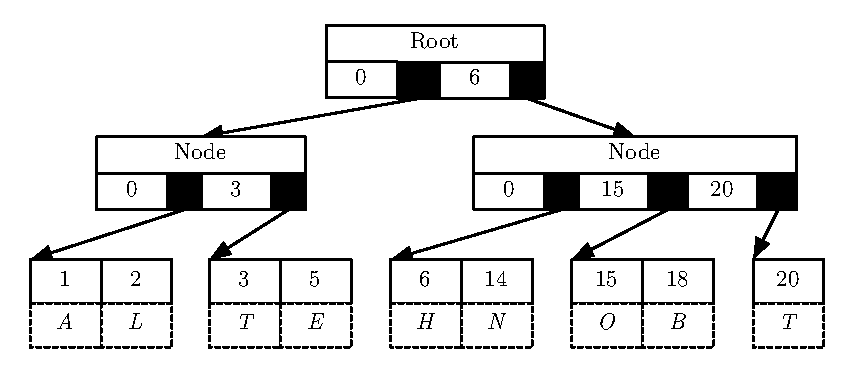
\includegraphics[width=90mm]{diagrams/BPlusTreeImpl.pdf}
 \caption{The same B+ tree as in Figure \ref{fig:bplustree} but with our specific list implementation.}
 \label{fig:bplustreeImpl}
\end{figure}

Figure \ref{fig:bplustree} shows that for each node with $n$ keys there are $n+1$ pointers to sub trees. As it can be seen from both Figure \ref{fig:inductive_data_type} and \ref{fig:bplustreeImpl} we have chosen to deal with this asymmetry by always having an explicit $0$ key in the beginning of each key-pointer list, such that a node with $n$ keys has $n$ pointers. Another way to represent a node would be to have $n$ key-pointer pairs as well as a start pointer of the type \begin{coqdoccode}\coqdocvar{bplustree} \coqdocvar{b} \coqdocvar{X}\end{coqdoccode}. However, that would give us unnecessary complexity both when writing our primary functions but also when proving theorems about these functions. Even though it is more strongly typed with such a definition we would always have to take care of a start pointer corner case when proving anything about our B+ trees. With our current solution we add a couple of assumptions to our notion of what a valid B+ tree is, to ensure the start pointer is properly handled. This will be explained in Section \ref{subsec:Valid_bplustree}. \todo{Maybe write that our implementation has at most $2b+1$ key-pointer pairs and at least $b+1$}

\paragraph{}
This functional implementation of B+ trees, which is an inherently imperative data structure, does have some implications. A popular implementation of nodes and leaves entails representing the key-pointer and key-value pairs as an array as it enables the fast binary search which runs in $O(log(n))$. Since Gallina does not support arrays, the only way to get lookups in key-pointer and key-value faster than $O(n)$ is through a tree structure, such as a B+ tree. This would add a large degree of complexity to our proofs, and since running time is not an objective of this project, it has been deemed out of scope.

\subsection{Valid B+ tree}
\label{subsec:Valid_bplustree}
Although the inductive data type can represent a B+ tree, it says nothing about the validity of a tree. It is entirely possible to build B+ trees that break the constraints from Section \ref{subsec:Background_Bplus_tree} using the $bplustree$ data type. To make statements about a B+ tree's validity, and to be sure that the trees we are working with are valid, we need a proposition that states what must hold for a B+ tree to be valid. This proposition is called $valid\_bplustree$, and can be seen in Figure \ref{fig:inductive_valid_bplustree}.

\begin{figure}
\centering
\begin{coqdoccode}
\coqdockw{Inductive} \coqdocvar{valid\_bplustree} (\coqdocvar{b}: \coqdocvar{nat}) (\coqdocvar{X}: \coqdockw{Type}) : \coqdocvar{bplustree} \coqdocvar{b} \coqdocvar{X} \ensuremath{\rightarrow} \coqdockw{Prop} :=\coqdoceol
\coqdocindent{1.00em}
\ensuremath{|} \coqdocvar{root\_is\_a\_leaf}  : \coqdockw{\ensuremath{\forall}} (\coqdocvar{kvl}: \coqdocvar{list} (\coqdocvar{nat} \ensuremath{\times} \coqdocvar{X})), \coqdoceol
\coqdocindent{11.00em}
\coqdocvar{b} \ensuremath{\not=} 0 \ensuremath{\rightarrow}\coqdoceol
\coqdocindent{11.00em}
\coqdocvar{length} \coqdocvar{kvl} \ensuremath{\le} \coqdocvar{b} \ensuremath{\times} 2 \ensuremath{\rightarrow}\coqdoceol
\coqdocindent{11.00em}
\coqdocvar{kvl\_sorted} \coqdocvar{kvl} \ensuremath{\rightarrow}  \coqdoceol
\coqdocindent{11.00em}
\coqdocvar{valid\_bplustree} \coqdocvar{b} \coqdocvar{X} (\coqdocvar{bptLeaf} \coqdocvar{b} \coqdocvar{X} \coqdocvar{kvl})\coqdoceol
\coqdocindent{1.00em}
\ensuremath{|} \coqdocvar{valid\_root\_node} : \coqdockw{\ensuremath{\forall}} (\coqdocvar{kpl}: \coqdocvar{list} (\coqdocvar{nat} \ensuremath{\times} \coqdocvar{bplustree} \coqdocvar{b} \coqdocvar{X})),\coqdoceol
\coqdocindent{11.00em}
\coqdocvar{b} \ensuremath{\not=} 0 \ensuremath{\rightarrow} \coqdoceol
\coqdocindent{11.00em}
2 \ensuremath{\le} \coqdocvar{length} \coqdocvar{kpl} \ensuremath{\rightarrow} \coqdoceol
\coqdocindent{11.00em}
\coqdocvar{length} \coqdocvar{kpl} \ensuremath{\le} \coqdocvar{S} (\coqdocvar{b} \ensuremath{\times} 2) \ensuremath{\rightarrow}\coqdoceol
\coqdocindent{11.00em}
\coqdocvar{key\_at\_index} 0 \coqdocvar{kpl} = \coqdocvar{Some} 0 \ensuremath{\rightarrow} \coqdoceol
\coqdocindent{11.00em}
\coqdocvar{all\_values} (\coqdocvar{bplustree} \coqdocvar{b} \coqdocvar{X}) (\coqdocvar{valid\_sub\_bplustree} \coqdocvar{b} \coqdocvar{X}) \coqdocvar{kpl} \ensuremath{\rightarrow}\coqdoceol
\coqdocindent{11.00em}
\coqdocvar{all\_values\_eq\_prop} (\coqdocvar{bplustree} \coqdocvar{b} \coqdocvar{X}) \coqdocvar{equal\_height} \coqdocvar{kpl} \ensuremath{\rightarrow}\coqdoceol
\coqdocindent{11.00em}
\coqdocvar{kvl\_sorted} \coqdocvar{kpl} \ensuremath{\rightarrow}  \coqdoceol
\coqdocindent{11.00em}
\coqdocvar{valid\_splits} \coqdocvar{b} \coqdocvar{X} \coqdocvar{kpl} \ensuremath{\rightarrow}\coqdoceol
\coqdocindent{11.00em}
\coqdocvar{valid\_bplustree} \coqdocvar{b} \coqdocvar{X} (\coqdocvar{bptNode} \coqdocvar{b} \coqdocvar{X} \coqdocvar{kpl})   \coqdoceol
\end{coqdoccode}
\caption{Inductive data type for a valid B+ tree.}
\label{fig:inductive_valid_bplustree}
\end{figure}

This proposition is only valid when examining the root of a tree, as there are different constraints for subtrees (See Section \ref{subsec:Background_Bplus_tree}). $valid\_bplustree$ has two cases, the first holds when the root of the B+ tree is a leaf, and the second holds when the root is a node. The various properties that must hold are explained below.

\paragraph{Root is a leaf}
The following must hold for a root leaf to be a valid B+ tree:
\label{valid_root_is_a_leaf}
\begin{itemize}
\item $b \neq 0$ --- The order must not be 0. Since we are working with natural numbers, this means $b > 0$.
\item $length\ kvl \leq b \times 2 $ --- The leaf must have at most $2b$ elements.
\item $kvl\_sorted\ kvl$ --- The keys in the leaf must be sorted.
\end{itemize}

\paragraph{Root is a node}
The following must hold for a root node to be a valid B+ tree:
\label{valid_root_is_a_node}
\begin{itemize}
\item $b \neq 0$ --- The order must not be 0.
\item $2 \leq length\ kpl$ and $length\ kpl \leq S\ (b \times 2)$ --- These satisfy the conditions for order stated in Section \ref{subsec:Background_Bplus_tree}.
\item $key\_at\_index\ 0\ kpl = Some\ 0$ --- As mentioned above, we must know that the first key is always 0. This assures that this is the case.
\item $all\_values (bplustree\ b\ X)\ (valid\_sub\_bplustree\ b\ X)\ kpl$ --- All the values stored in the node (the pointers) must be valid subtrees. As mentioned in Section \ref{subsec:Background_Bplus_tree}, the constraints for the root are slightly different. The constraints for internal leaves and nodes will be covered below.
\item $all\_values\_eq\_prop (bplustree\ b\ X)\ equal\_height\ kpl$ --- All subtrees must have the same height.
\item $kvl\_sorted\ kpl$ --- The keys in the node must be sorted.
\item $valid\_splits\ b \ X\ kpl$ --- All the splits are correct, i.e. all the keys in a subtree are between the keys of its siblings.
\end{itemize}

\paragraph{}
Since $valid\_bplustree$ only holds for the root leaf or node, a different proposition is needed for non-root leaves and nodes, or subtrees. This is implemented in the $valid\_sub\_bplustree$ proposition. In the interest of brevity, only the differences will be listed here:

\paragraph{Non-root leaf}
\begin{itemize}
\item $b \leq length\ kvl$ --- The number of key-value pairs in the leaf must be at least $b$.
\end{itemize}

\paragraph{Non-root node}
\begin{itemize}
\item $2 \leq length\ kpl$ changed to $S\ b \leq length\ kpl$ --- The number of key-pointer pairs must be at least $b+1$.
\end{itemize}

Now both a data type for B+ trees, and a way to reason about their validity have been defined. With the the $bplustree$ data type we can start implementing the search and insert functions, and $valid\_bplustree$ gives us the assumptions that are needed for proving facts about these functions.

\subsection{Search}
\label{subsec:search}
Our implementation of search does not stray far from the prototypical version described in the background (Section \ref{sec:Background}). It is implemented through 3 functions: $search'$, $find\_subtree$, and $search\_leaf$. 
\todo{Write about sorted}

\paragraph{}
Both our $insert$ and $search$ are recursive function recursing over a descending parameter $counter$. The reason for introducing this parameter is to serve as a recursion terminator. Because our inductive type for B+ trees consists of a nesting of two inductive datatypes that are not mutually recursive, Coq is unable to reason about instances of $bplustree$ has a recursively decreasing argument. Since a key requirement for recursive Coq functions is that they must contain a decreasing argument, we introduced this notion of a counter that we will decrease by one every time we decent one down to a subtree. If the counter ever reaches $0$, the recursion stops. This means that should the counter ever reach $0$ before we have descended all the way down the tree, a wrong result will be given. To ensure this never happens, we always initialize the counter to the height of the tree.

The reason why initializing the counter to the height of the tree will guarantee that our counter will never reach $0$ before our $insert'$ implementation have descended all the way down to a leaf is simple. Our implementation of $height$ simply counts the number of steps it takes to descend down the leftmost child in every node until it reaches a leaf. Our $valid\_bplustree$ proposition captures the balancing nature of B+trees so if $height$ is called on such a valid B+ tree, the returned valid is the number of steps from the root to any leaf in the tree. So irregardless of which leaf the insert must happen in, we know we can decend that far down the tree in $counter$ steps. Because our implementation of $insert'$ only decreases the counter by one every time it recursively call itself with a subtree, we have a invariant where the counter will always be exactly equal to the height of the tree it currently processing. This invariant is a key aspect to constructing induction proofs on our B+ trees with our implementation doesn't have a datatype that is not inductively defined over the height of the tree.

\paragraph{}
A key part of both insertion and searching in our implementation is the function $find\_subtree$. This function, when given a list of key-pointer pair, and a search-key, will identify the key-pointer pair whose range contains the search-key. The pointer in the identified key-pointer pair is the subtree that, in a valid B+ tree, must contain the search-key if the tree contains the key.

\paragraph{}
The main function that performs search is $search'$, that as mentioned above is recursively defined over a natural number counter. It uses $find\_subtree$ to identify which subtree to recurse into, and when it reaches a leaf it calls $search\_leaf$. $search\_leaf$ performs a simple linear search through the key-value pairs to identify if the search-key exists within the tree.

To ensure that the counter is always initialized to the height of the tree to search, we have added a definition of $search$ that simply calls $search'$ with the $counter = height(tree)$.

\subsection{Insert}
The $insert$ function calls the $insert'$ function to insert into a tree. First $insert'$ recurses down through $counter$ layers to find the insertion point, after which it handles overflow, if any should occur, on the way back up through the recursion layers. The function $insert'$ never increases the height of the tree but lets $insert$ handle the case where the root node overflows. In this case $insert$ will split the former root node into two sub nodes and connect these to a new root. This case obviously increases the height of the tree by $1$ and keeps the tree balanced. Effectively, this means the invariant described in Section \ref{subsec:search} still holds for $insert'$, as the height of the balanced tree is always equal to the $counter$ variable, which the $insert'$ function is decreasing on.
\paragraph{}
Out of the three central $insert$, $insert'$ and $insert\_leaf$ functions the significant is $insert'$. It uses $find\_subtree$ to figure out which subtree it should recurse into and $insert\_node$ to handle overflowing subtrees. Where $insert'$ handles overflowing leafs, $insert\_node$ takes care of overflowing (non-root) nodes.

\subsection{Elements of a Complete Proof of Correctness}
\todo{Use coqdoc in this section}
For insertion and search, a formal verification of the implementations would entail a combination of three different (but related) main proofs.
\subsubsection{InsertSearchWorks}
Whenever we insert into a tree with insert, we should be able to find it again afterwards. This is true even in the case where the key already exists and we have to overwrite the value. The proposition looks the following way: $search\ k\ (insert\ k\ v\ t) = Some\ v$, and it can be found in InsertSearchWorksProofs.v.
\subsubsection{InsertPreserves}
It is, however, not enough to just show that an inserted element is retrievable. It says nothing about the validity of the tree and thus the insertion function could easily leave the tree unbalanced or otherwise invalid. With the definition of a valid B+ tree from Section \ref{subsec:Valid_bplustree}, we can define the following proposition that must hold: $valid\_bplustree\ b\ X\ tree\ \rightarrow valid\_bplustree\ b\ X\ (insert\ k\ v\ tree)$. It can be found in InsertPreservesProofs.v.
\subsubsection{InsertPreservesElements}
As a final guard we must ensure that insert does not throw away elements from the initial tree or inserts other elements. A flawed implementation of insert, designed to circumvent the two above-mentioned proofs, could just return a leaf with the inserted key-value pair for all trees. By using an in-order traversal of the tree, together with a simple insertion into the sorted list it produces, we can ensure that no elements are lost, and that only the $(k, v)$ pair is inserted. In its simplest form it is structured the following way: $insert_into_list k v (inorder t) = inorder (insert k v t)$. See InsertPreservesElements.v for the full specification of the proof. 
\subsubsection{Scope and Proof Limitations}
Proving these three main theorems in Coq is an immense task. As a consequence, we have chosen to focus on the most central one, which is the InsertSearchWorks proof, as it is the most heavily depended upon of the three, as it only holds if all the primary functions are correct. 
\paragraph{}
However, as mentioned above, only proving InsertSearchWorks leaves the possibility for a incorrect implementation of insert that just throws away the initial tree and returns a leaf with the inserted element. We will let it be up to the reader to verify that our insertion function is not implemented that way, and so we list InsertPreservesElements as future work. Conversely, the assumption that the insertion function ensures that the validity of the tree is preserved is much more difficult to manually verify. Not having proved InsertPreserves is a central admission in the proof of InsertSearchWorks, as the search function assumes that the input tree is valid. Given the fact that we currently do not ensure that the tree is valid after insertion, we cannot prove that the input tree handed to the search function (in our InsertSearchWorks proof) is actually valid. InsertPreserves is classified as future work as well.

%!TEX root = ../BPlusTree-report.tex
\section{Proof Realization}
\label{sec:ProofRealization}
% Notes:
% bplustree inductive datatype
%   - Why not have a start pointer/end pointer?
% insert/search
%   - Use appears_in instead of search(insert)
% insert
%   - mutually recursive
%   - Kopitiam cannot handle large proof assumptions
%   -counter
In this section, 

\subsection{Proofs about sortedness}
A vital aspect of B+ trees is that all of the key-point and key-value lists in nodes and leafs are sorted by key. So the first proposition we defined was $kvl\_sorted$ that is only applicable to such sorted lists. The proposition can be seen reproduced in figure \ref{fig:kvl_sorted}.

\begin{figure}
  \begin{coqdoccode}
  \coqdocnoindent
  \coqdockw{Inductive} \coqdocvar{kvl\_sorted} \{\coqdocvar{X}: \coqdockw{Type}\}: \coqdocvar{list} (\coqdocvar{nat} \ensuremath{\times} \coqdocvar{X}) \ensuremath{\rightarrow} \coqdockw{Prop} :=\coqdoceol
  \coqdocindent{2.00em}
  \coqdocvar{kvl\_sorted\_0}: \coqdocvar{kvl\_sorted} []\coqdoceol
  \coqdocindent{1.00em}
  \ensuremath{|} \coqdocvar{kvl\_sorted\_1}: \coqdockw{\ensuremath{\forall}} (\coqdocvar{n}: \coqdocvar{nat}) (\coqdocvar{x}: \coqdocvar{X}), \coqdoceol
  \coqdocindent{8.00em}
  \coqdocvar{kvl\_sorted} [(\coqdocvar{n}, \coqdocvar{x})]\coqdoceol
  \coqdocindent{1.00em}
  \ensuremath{|} \coqdocvar{kvl\_sorted\_cons}: \coqdockw{\ensuremath{\forall}} (\coqdocvar{n1} \coqdocvar{n2}: \coqdocvar{nat}) (\coqdocvar{x1} \coqdocvar{x2}: \coqdocvar{X}) (\coqdocvar{lst}: \coqdocvar{list} (\coqdocvar{nat} \ensuremath{\times} \coqdocvar{X})), \coqdoceol
  \coqdocindent{8.00em}
  \coqdocvar{kvl\_sorted} ((\coqdocvar{n2},\coqdocvar{x2})::\coqdocvar{lst}) \ensuremath{\rightarrow} \coqdoceol
  \coqdocindent{8.00em}
  \coqdocvar{blt\_nat} \coqdocvar{n1} \coqdocvar{n2} = \coqdocvar{true} \ensuremath{\rightarrow}\coqdoceol
  \coqdocindent{8.00em}
  \coqdocvar{kvl\_sorted} ((\coqdocvar{n1},\coqdocvar{x1})::(\coqdocvar{n2},\coqdocvar{x2})::\coqdocvar{lst}).\coqdoceol
  \end{coqdoccode}
  \caption{Our proposition about sorting}
  \label{fig:kvl_sorted}
\end{figure}

Because almost all of our proofs entails manipulating sorted list, we first built up a extensive set of lemmas and theorems detailing how the proposition behaves when the list is changed -- e.g. if you remove the head of the list, the remainder is still sorted. We have reproduced a few of these behaviors in figure \ref{fig:key_sorting_lemmas}. The theorem $insert\_preserves\_sort$ is probably the one with most direct impact to the rest of the proofs. This is the lemma that allows us to insert new items into a key-value or key-pointer list and know that the list continues to be sorted. $sort\_ignores\_values$ simply confirms that our sorting is only concerned with the keys in the list, as we can swab out one key for another without impacting the validity of the proposition. $list\_tail\_is\_sorted$ is a very handy lemma when dealing with induction over lists, because it quickly allows us to pop the head element off a list and still know that the resulting list is sorted.

\begin{figure}
  \begin{coqdoccode}
  \coqdocnoindent
  \coqdockw{Lemma} \coqdocvar{sort\_ignores\_value} : \coqdockw{\ensuremath{\forall}} (\coqdocvar{X}: \coqdockw{Type}) (\coqdocvar{k}: \coqdocvar{nat}) (\coqdocvar{v1} \coqdocvar{v2}: \coqdocvar{X}) (\coqdocvar{l}: \coqdocvar{list} (\coqdocvar{nat} \ensuremath{\times} \coqdocvar{X})),\coqdoceol
  \coqdocindent{1.00em}
  \coqdocvar{kvl\_sorted} ((\coqdocvar{k},\coqdocvar{v1})::\coqdocvar{l}) \ensuremath{\rightarrow} \coqdocvar{kvl\_sorted}((\coqdocvar{k}, \coqdocvar{v2})::\coqdocvar{l}).\coqdoceol
  \coqdocemptyline
  \coqdocnoindent
  \coqdockw{Lemma} \coqdocvar{list\_tail\_is\_sorted} : \coqdockw{\ensuremath{\forall}} (\coqdocvar{X}: \coqdockw{Type}) (\coqdocvar{l}: \coqdocvar{list} (\coqdocvar{nat} \ensuremath{\times} \coqdocvar{X})) (\coqdocvar{k}: \coqdocvar{nat}) (\coqdocvar{v}: \coqdocvar{X}),\coqdoceol
  \coqdocindent{1.00em}
  \coqdocvar{kvl\_sorted} ((\coqdocvar{k},\coqdocvar{v})::\coqdocvar{l}) \ensuremath{\rightarrow} \coqdocvar{kvl\_sorted} \coqdocvar{l}.\coqdoceol
  \coqdocemptyline
  \coqdocnoindent
  \coqdockw{Lemma} \coqdocvar{kvl\_sorted\_key\_across\_app} : \coqdockw{\ensuremath{\forall}} (\coqdocvar{X}: \coqdockw{Type}) (\coqdocvar{l1} \coqdocvar{l2}: \coqdocvar{list} (\coqdocvar{nat} \ensuremath{\times} \coqdocvar{X})) (\coqdocvar{k1} \coqdocvar{k2}: \coqdocvar{nat}) (\coqdocvar{v1} \coqdocvar{v2}: \coqdocvar{X}),\coqdoceol
  \coqdocindent{1.00em}
  \coqdocvar{kvl\_sorted}((\coqdocvar{k1}, \coqdocvar{v1})::\coqdocvar{l1} ++ (\coqdocvar{k2}, \coqdocvar{v2})::\coqdocvar{l2}) \ensuremath{\rightarrow} \coqdocvar{k1} < \coqdocvar{k2}.\coqdoceol
  \coqdocemptyline
  \coqdocnoindent
  \coqdockw{Theorem} \coqdocvar{insert\_preserves\_sort} : \coqdockw{\ensuremath{\forall}} (\coqdocvar{X}: \coqdockw{Type}) (\coqdocvar{l}: \coqdocvar{list} (\coqdocvar{nat} \ensuremath{\times} \coqdocvar{X})) (\coqdocvar{k}: \coqdocvar{nat}) (\coqdocvar{v}: \coqdocvar{X}),\coqdoceol
  \coqdocindent{1.00em}
  \coqdocvar{kvl\_sorted} \coqdocvar{l} \ensuremath{\rightarrow} \coqdocvar{kvl\_sorted} (\coqdocvar{insert\_into\_list} \coqdocvar{k} \coqdocvar{v} \coqdocvar{l}).\coqdoceol
  \coqdocemptyline
  \end{coqdoccode}
  \caption{Key lemmas and theorems about sorting}
  \label{fig:key_sorting_lemmas}
\end{figure}

\subsection{Intermediate proposition}

We have chosen to prove the correctness of our implementation using a added level of indirection. Instead of directly proving that $search k (insert k v tree) = Some v$, we are instead proving after inserting into a tree, we know that the tree has a certain property -- that it contains the inserted key --. Likewise we prove that if this proposition holds for a tree, then $search$ can retrieve the item.

\subsubsection{Reasoning about contents}
To verify that our solution can search and insert into both leafs and entire trees, we designed two propositions that allows us to reason about the content of leafs and trees. The two propositions can be seen represented in figure \ref{fig:aik_and_ait}. 

\begin{figure}
\centering
\begin{coqdoccode}
  \coqdocnoindent
  \coqdockw{Inductive} \coqdocvar{appears\_in\_kvl} \{\coqdocvar{X}:\coqdockw{Type}\} (\coqdocvar{sk}: \coqdocvar{nat}) : \coqdocvar{list} (\coqdocvar{nat} \ensuremath{\times} \coqdocvar{X}) \ensuremath{\rightarrow} \coqdockw{Prop} :=\coqdoceol
  \coqdocindent{1.00em}
  \ensuremath{|} \coqdocvar{aik\_here}: \coqdockw{\ensuremath{\forall}} \coqdocvar{v} \coqdocvar{l},		~~~\coqdocvar{appears\_in\_kvl} \coqdocvar{sk} ((\coqdocvar{sk}, \coqdocvar{v})::\coqdocvar{l})\coqdoceol
  \coqdocindent{1.00em}
  \ensuremath{|} \coqdocvar{aik\_later}: \coqdockw{\ensuremath{\forall}} \coqdocvar{k} \coqdocvar{v} \coqdocvar{l},	\coqdocvar{appears\_in\_kvl} \coqdocvar{sk} \coqdocvar{l} \ensuremath{\rightarrow} \coqdocvar{appears\_in\_kvl} \coqdocvar{sk} ((\coqdocvar{k}, \coqdocvar{v})::\coqdocvar{l}).\coqdoceol
  \coqdocemptyline
  \coqdocnoindent
  \coqdockw{Inductive} \coqdocvar{appears\_in\_tree} \{\coqdocvar{X}:\coqdockw{Type}\} \{\coqdocvar{b}: \coqdocvar{nat}\} (\coqdocvar{sk}: \coqdocvar{nat}) : \coqdocvar{bplustree} \coqdocvar{b} \coqdocvar{X} \ensuremath{\rightarrow} \coqdockw{Prop} :=\coqdoceol
  \coqdocindent{1.00em}
  \ensuremath{|} \coqdocvar{ait\_leaf}: \coqdockw{\ensuremath{\forall}} \coqdocvar{l},	~~\coqdocvar{appears\_in\_kvl} \coqdocvar{sk} \coqdocvar{l} \ensuremath{\rightarrow} \coqdocvar{appears\_in\_tree} \coqdocvar{sk} (\coqdocvar{bptLeaf} \coqdocvar{b} \coqdocvar{X} \coqdocvar{l})\coqdoceol
  \coqdocindent{1.00em}
  \ensuremath{|} \coqdocvar{ait\_node\_last}: \coqdockw{\ensuremath{\forall}} \coqdocvar{k1} \coqdocvar{k2} \coqdocvar{v1} \coqdocvar{v2}, \coqdoceol
  \coqdocindent{8.00em}
  \coqdocvar{appears\_in\_tree} \coqdocvar{sk} \coqdocvar{v2} \ensuremath{\rightarrow} \coqdocvar{k2} \ensuremath{\le} \coqdocvar{sk} \ensuremath{\rightarrow}\coqdoceol
  \coqdocindent{8.00em}
  \coqdocvar{appears\_in\_tree} \coqdocvar{sk} (\coqdocvar{bptNode} \coqdocvar{b} \coqdocvar{X} [(\coqdocvar{k1}, \coqdocvar{v1}), (\coqdocvar{k2}, \coqdocvar{v2})])\coqdoceol
  \coqdocindent{1.00em}
  \ensuremath{|} \coqdocvar{ait\_node\_here}: \coqdockw{\ensuremath{\forall}} \coqdocvar{k1} \coqdocvar{k2} \coqdocvar{v1} \coqdocvar{v2} \coqdocvar{l}, \coqdoceol
  \coqdocindent{8.00em}
  \coqdocvar{appears\_in\_tree} \coqdocvar{sk} \coqdocvar{v1} \ensuremath{\rightarrow} \coqdocvar{k1} \ensuremath{\le} \coqdocvar{sk} \ensuremath{\land} \coqdocvar{sk} < \coqdocvar{k2} \ensuremath{\rightarrow}\coqdoceol
  \coqdocindent{8.00em}
  \coqdocvar{appears\_in\_tree} \coqdocvar{sk} (\coqdocvar{bptNode} \coqdocvar{b} \coqdocvar{X} ((\coqdocvar{k1}, \coqdocvar{v1})::(\coqdocvar{k2}, \coqdocvar{v2})::\coqdocvar{l}))\coqdoceol
  \coqdocindent{1.00em}
  \ensuremath{|} \coqdocvar{ait\_node\_later}: \coqdockw{\ensuremath{\forall}} \coqdocvar{x} \coqdocvar{k1} \coqdocvar{k2} \coqdocvar{v1} \coqdocvar{v2} \coqdocvar{l},\coqdoceol
  \coqdocindent{8.00em}
  \coqdocvar{appears\_in\_tree} \coqdocvar{sk} (\coqdocvar{bptNode} \coqdocvar{b} \coqdocvar{X} ((\coqdocvar{k1}, \coqdocvar{v1})::(\coqdocvar{k2}, \coqdocvar{v2})::\coqdocvar{l})) \ensuremath{\rightarrow} \coqdoceol
  \coqdocindent{8.00em}
  \coqdocvar{k1} \ensuremath{\le} \coqdocvar{sk} \ensuremath{\rightarrow}\coqdoceol
  \coqdocindent{8.00em}
  \coqdocvar{appears\_in\_tree} \coqdocvar{sk} (\coqdocvar{bptNode} \coqdocvar{b} \coqdocvar{X} (\coqdocvar{x}::(\coqdocvar{k1}, \coqdocvar{v1})::(\coqdocvar{k2}, \coqdocvar{v2})::\coqdocvar{l})).\coqdoceol
  \end{coqdoccode}
\caption{Inductive propositions for reasoning about contents}
\label{fig:aik_and_ait}
\end{figure}

We can reason about leafs using the $appears\_in\_kvl$ proposition on the leafs key-value pairs. If a key is present in the list, then the proposition holds. Likewise the list can not contain a given key if the proposition does not hold. We use this property in our proofs of that $search\_leaf$ and $insert\_leaf$. To proof that $search\_leaf$ works, we must simply prove that \begin{coqdoccode} 
  \coqdocvar{appears\_in\_kvl} \coqdocvar{k} \coqdocvar{kvl}
  \ensuremath{\rightarrow} \coqdocvar{\ensuremath{\exists}} \coqdocvar{v}, 
  \coqdocvar{search\_leaf} \coqdocvar{k} \coqdocvar{kvl} = \coqdocvar{Some} 
  \coqdocvar{v}
\end{coqdoccode} holds. Or to paraphrase, if a given key exists in the key-value list, then there must exists a value that $search\_leaf$ finds if we search for that key. In reality we must also know that the key-value list is sorted, so the actual proof also reflects this requirement.

Similarly the proof for ensuring that $insert\_leaf$ can be seen as \begin{coqdoccode}
\ensuremath{\lnot} \coqdocvar{appears\_in\_kvl} \coqdocvar{k} \coqdocvar{kvl} \ensuremath{\rightarrow} \coqdocvar{appears\_in\_kvl} \coqdocvar{k} (\coqdocvar{insert\_leaf} \coqdocvar{k} \coqdocvar{v} \coqdocvar{kvl})
\end{coqdoccode}. But because calling $insert\_leaf$ can overflow the leaf, the return type of $insert\_leaf$ is not $list(nat * X)$, but rather $(list (nat * X) * option (list (nat * X)))$. So it $insert\_leaf$ returns a key-value list and a option for the portion of the key-value list that overflowed. So the actual lemma is a disjunction stating that they key must appear in one of the two returned key-value lists.

\paragraph{}
To reason about entire trees, we have the the proposition $appears\_in\_tree$. The proposition has a single constructor for when the tree is a leaf, where the only requirement is that $appears\_in\_kvl$ must hold for the leafs key-value list. When the tree is a node, we have three different constructors. We have two constructors ($ait\_node\_last$ and $ait\_node\_here$) for when the the key should appear in a specific subtree, and one ($ait\_node\_later$) that allows you to add subtrees that should not contain the search-key.

Like with leafs, we use $appears\_in\_kvl$ on the key-pointer list and then prove properties about $search$ and $insert$. The two theorems can be seen reproduced in figure \ref{fig:search_works} and \ref{fig:insert_works}.







\subsection{Reasoning about search}
We want to prove that $search$ actually performs like we expect it to. So if a key is present in a tree, we expect $search$ to find a value. Likewise we expect $search$ to not find anything when the key is not present in the tree.
some of the above should be moved here. Put more succinctly, we must prove that $appears\_in\_tree~k~tree \rightarrow \exists v, search~k~tree = Some~v$ and $\lnot appears\_in\_tree~k~tree \rightarrow search~k~tree = None$.

\begin{figure}
  \begin{coqdoccode}
  \coqdocnoindent
  \coqdockw{Theorem} \coqdocvar{appears\_search\_works} : \coqdockw{\ensuremath{\forall}} (\coqdocvar{b}: \coqdocvar{nat}) (\coqdocvar{X}: \coqdockw{Type}) (\coqdocvar{t}: \coqdocvar{bplustree} \coqdocvar{b} \coqdocvar{X}) (\coqdocvar{k}: \coqdocvar{nat}),\coqdoceol
  \coqdocindent{1.00em}
  \coqdocvar{valid\_bplustree} \coqdocvar{b} \coqdocvar{X} \coqdocvar{t} \ensuremath{\rightarrow} \coqdoceol
  \coqdocindent{1.00em}
  \coqdocvar{appears\_in\_tree} \coqdocvar{k} \coqdocvar{t} \ensuremath{\rightarrow} \coqdoceol
  \coqdocindent{1.00em}
  \coqdocvar{\ensuremath{\exists}} \coqdocvar{v}, \coqdocvar{search} \coqdocvar{k} \coqdocvar{t} = \coqdocvar{Some}(\coqdocvar{v}).\coqdoceol
  \end{coqdoccode}
  \caption{The theorems that claim that $search$.}
  \label{fig:search_works}
\end{figure}

\subsection{Insert impl. appears}
some of the above should be moved here and find\_subtree must always find a subtree

\begin{figure}
  \begin{coqdoccode}
  \coqdocnoindent
  \coqdockw{Theorem} \coqdocvar{insert\_works} : \coqdockw{\ensuremath{\forall}} \{\coqdocvar{X}: \coqdockw{Type}\} \{\coqdocvar{b}: \coqdocvar{nat}\} (\coqdocvar{t}: \coqdocvar{bplustree} \coqdocvar{b} \coqdocvar{X}) (\coqdocvar{k}: \coqdocvar{nat}) (\coqdocvar{v}: \coqdocvar{X}),\coqdoceol
  \coqdocindent{1.00em}
  \coqdocvar{valid\_bplustree} \coqdocvar{b} \coqdocvar{X} \coqdocvar{t} \ensuremath{\rightarrow} \coqdoceol
  \coqdocindent{1.00em}
  \ensuremath{\lnot}\coqdocvar{appears\_in\_tree} \coqdocvar{k} \coqdocvar{t} \ensuremath{\rightarrow} \coqdoceol
  \coqdocindent{1.00em}
  \coqdocvar{appears\_in\_tree} \coqdocvar{k} (\coqdocvar{insert} \coqdocvar{k} \coqdocvar{v} \coqdocvar{t}).\coqdoceol
  \end{coqdoccode}
  \caption{The theorems that claim that $insert$ works.}
  \label{fig:insert_works}
\end{figure}

\subsection{Tying it together}
Fill me in.

%!TEX root = ../BPlusTree-report.tex
\section{Evaluation}
\label{sec:Evaluation}
Formally verifying a non-trivial data type like B+ trees has proven to be a difficult task. In this section we evaluate four central points regarding our work process and our $insert\_search\_works$ proof.

\subsubsection{Insert Into Leaf}
Our strategy for proving the $insert\_impl\_appears$ proof was to prove the base case separately. The base case is inserting into a tree with $height = 0$, or in other words a leaf. So the initial lemma we set out to prove was $insert\_leaf\_impl\_appears$. But because we had not attempted to verify the behaviors of insertion in nodes, we had some incorrect assumptions about what we should prove. One problem was that we did not make the goal very strong, so when we later had to apply the lemma in $insert\_impl\_appears$ we had to establish a great deal in our context before we could apply the lemma. When we later set out to verify $insert'$, we improved this aspect and verified a much stronger statement.

\subsubsection{Unnecessary Assumption}
Another shortcoming in our initial assumptions when verifying $insert\_leaf\_impl\_appears$ was that the key was not present before insertion. As a result, our verification of insertion into leaves has the requirement that $\lnot appears\_in\_kvl$ must hold. Because we rely on the verification for leaves when verifying insertion in trees, this assumption bubbles up and adds the requirement that $\lnot appears\_in\_tree$ must hold before inserting. In retrospect this assumption is unnecessary, and results in a slightly weaker verification. We have only verified that inserting a new value works, not that overwriting an existing key works too. 

\subsubsection{Higher Priority for Validity Preservation Proof}

With a better overview we might have chosen to prove \textit{insert\allowbreak{}\_preserves\allowbreak{}\_validity} first. Our \textit{insert\allowbreak{}\_search\allowbreak{}\_works} proof relies on insertion preserving the validity, so without verification of this preservation we can not create a complete verification that inserted items can be found. The way we have structured our proofs means that it is only in the final lemma we require this preservation, so our two intermediate theorems are fully verified.

The reason why we chose to verify \textit{insert\_search\_works} first, is that that we felt that a such verification was more telling of our actual implementation rather than proving that we maintained a inductively defined proposition. The verification of $insert$ and $search$ relies on all aspects of our B+ tree implementation and because of our structure with the intermediate proposition, we only had to use the validity preservation at the very end.

\subsubsection{The Use of Booleans}

Within our implementation we rely heavily on the use of $bool$ when comparing natural numbers (i.e. $beq\_nat$, $ble\_nat$ and $blt\_nat$) and performing conjunctions (i.e. $andb$). In retrospect this is unnecessary and convoluted the verification because of all the required conversions from $bool$ to $Prop$. It would likely have been simpler had we used $Either$ instead.

\subsubsection{Unverified Claims}

As mentioned in Section \ref{sec:ElementsOfACompleteProof}, we have limited the scope of this assignment to only cover the main theorem $insert\_search\_works$. This means that the two other theorems ($insert\allowbreak{}\_preserves\allowbreak{}\_elements$ and $insert\allowbreak{}\_preserves\allowbreak{}\_tree\allowbreak{}\_validity$) are completely unverified.

Because $insert\_search\_works$ relies on $insert\_preserves\_tree\_validity$ for it's final step, we can not claim to have completely verified this theorem. We have however individually verified the two theorems around our intermediate proposition.

%!TEX root = ../BPlusTree-report.tex
\section{Related Work}
\label{sec:RelatedWork}
Sexton et al.\,\cite{sexton2008reasoning} use an abstract machine to specify operations on B+ trees, and then use separation logic to reason about these operations, specifically the insert and range query operations. Their approach lets them reason locally about the subtree being modified, while the rest of the tree is invariant. This makes their proofs less complex, as they only have to take a small part of the tree into account. It should be noted that their work does not constitute a formal proof, but rather a rigorous informal proof.

\paragraph{}
Ernst et al.\,\cite{ernst2011verification} use the TVLA tool to conduct shape analysis on B+ trees, automatically discharching many proof obligations related to the structure of B+ trees, such as proof of acyclicity, while using the KIV interactive proof assistant to prove move complicated obligations. They argue that automated shape analysis combined with interactive theorem proving is a great improvement over using one or the other alone.

\paragraph{}
Malecha et al.\,\cite{malecha2010toward} describe their formal verification of a light weight relational database management system including the B+ data structure. Using the Ynot extension for Coq to reason about imperative, pointer-based code they are capable of keeping the references between leaves effectively supporting range queries.

%!TEX root = ../BPlusTree-report.tex
\section{Conclusion}
\label{sec:Conclusion}
In this paper we presented a definition of B+ trees in Coq, and accounted for the performance and representational challenges connected to it. This included adding an extra zero key to the beginning of all nodes, as well as using the height of the given tree as a counter on which the insertion and search functions recursed. 
\paragraph{}
First we defined an inductive data type, called $valid\_bplustree~b~X$, for usage in various proofs related to the primary functions on B+ trees. Then we defined the three main theorems of a complete proof of correctness with regards to insertion and search. We decided to focus on $insert\_search\_works$, as we believed it to be the most significant of the three. As a consequence, we chose to leave $insert\_preserves\_tree\_validity$ and $insert\_preserves\_elements$ as future work.
\paragraph{}
To accommodate the need for reasoning about the search and insert functions independently, an intermediate proposition was defined. The $kv\_appears\_in\_tree$, $appears\_in\_tre$, $kv\_appears\_in\_kvl$, and $appears\_in\_kvl$ propositions were used to prove a list of facts that are informally described here:

\begin{itemize}
	\item If a key-value pair $(k, v)$ appears in a tree $t$ then $search~k~t = Some~(v)$
	\item If a key $k$ does not appear in a tree $t$ then $search~k~t = None$
	\item If the key of a key-value pair $(k, v)$ does not appear in a tree $t$, then performing $insert~k~v~t$ ensures that the pair appears in $t$.
\end{itemize} 

These facts were ultimately used to verify the correctness of InsertSearchWorks, the main theorem of the paper stating that subsequent insertion of a key-value pair and search of the same key-value pair would find it again.

%!TEX root = ../BPlusTree-report.tex
%\section{References}
%\label{sec:References}

\bibliography{BPlusTree-report}
%!TEX root = ../BPlusTree-report.tex
\appendix
\label{sec:Appendix}
\section{Running the code}
The code for this project is hosted on Github at \url{https://github.com/nicolaidahl/BPlusTrees}. The Coq implementation resides in the ./code/ subdirectory. A Makefile is provided that will build the project. It has been tested with Coq 8.3pl5 and later.


\end{document}
